\documentclass[a4paper]{article}

\usepackage[margin=1.2in]{geometry}
\usepackage{graphicx}
\usepackage{amsmath,amssymb,amsthm,bm}
\usepackage{latexsym,xcolor,minipage-marginpar,caption,multirow,verbatim}
\usepackage{enumerate}
\usepackage{titlesec}
\usepackage{mathtools}
\usepackage{pgfplots}


\begin{document}

\title{Homework 2 - Omer Ronen\\Stats 215A, Fall 2020
  }
\date{}
\maketitle
\vspace{-5em}

\begin{description}
\section{Principal Components Analysis and SVD}
\item[•]
\begin{enumerate}
\item{}
%\item[1. Principal Components Analysis and SVD]\hfill\\
First we define the Lagrangian
\[
L(v,\lambda) = v^{T}X^{T}Xv + \lambda (v^{T} v -1 )
\]
Next we take the derivatives
\[
\begin{aligned}
& \frac{\partial L}{\partial v} = 2 v^{T}X^{T}X + 2\lambda v^{T}\\
& \frac{\partial L}{\partial \lambda} = v^{T} v -1 
\end{aligned}
\]
Solving we first equation we have that
\[
v^{T}X^{T}X = \lambda v^{T}
\]
Which mean that $v$ is an eigen vector for the matrix $X^T X$ using the SVD of $X$ we note that $X^T X = VDU^{T} UDV^{T} = VD^{2}V^{T}$. We see that the columns of $V$ are the eigen vectors and $D^2$ is the diagonal matrix of the eigen values.\\
As each eigen vector is a stationary point for the problem, we note that for every eigen vector $v^{\star}$
\[
(v^{\star})^T X^T X v^{\star} = d^{\star}
\]
where $d^{\star}$ is the corresponding eigen value in $D^{2}$ matrix. Since we can assume that all values in $D$ are positive (if not we set $u_i' = - u_i$) this means that $v = v_1$.\\
\item{}
We know from the previous section that $X^T X =  VD^{2}V^{T}$, now let $v$ be any vector satisfying the conditions in the question then
\[
v^T X^T X v = v^T VD^{2}V^{T} v
\]
It's easy to to see that
\[
    h_j = (v^T VD)_i =v^T v_i
\]
And this vector is equal to zero for $i<j$. To conclude we simply note that 
\[
v^T X^T X v = h h^T  = \sum_{k=j}^{p} h_k h_k^T = \sum_{k=j}^{p} v^T (d_k^{2} v_k v_k^T) v
\]
\item{}
It is easy too see that when we plug in $X=X_{(j)}$ and repeat the same calculations as in (1) we would reach the same eigen value problem where we would select the eigen vector corresponding to the largest eigen value of $X_{(j)}^T X_{(j)}$\\
We prove the equivalence by induction, (1) is the induction basis, assume that $\hat{v_1}, \dots, \hat{v_{j-1}}$ are the eigen vectors corresponding to the $j-1$ largest eigen values of the matrix $X^T X$ and therefore solution to PC1-PCj-1 problems.\\
Let $v$ any feasible solution for the PCj problem, and note that the objective can be written as
\[
v^T X^T X v  = \sum_{h=j}^{p} \sum_{k=j}^{p} v^T ( v_h d_h d_k   v_k^T) v
\] 
Any feasible solution must be orthogonal to $\{v_1, \dots, v_{j-1}\}$ by the induction assumption, so $v^T\in \text{Span}(\{v_{j}, \dots, v_{p}  \})$ and we can write $v=\sum_{k=j}^{p} \alpha_k v_k;\; \sum_{k=j}^{p} \alpha_k = 1$, and see that
\[
\sum_{h=j}^{p} \sum_{k=j}^{p} v^T ( v_h d_h d_k   v_k^T) v = \sum_{h=j}^{p} \sum_{k=j}^{p} \sum_{n=j}^{p} \alpha_n \cdot \left(v_n^T ( v_h d_h d_k   v_k^T) v_n\right)
\]
By orthogonality this sum reduces to 
\[
\sum_{k=j}^{p}\alpha_k \cdot \left(v_k^T ( v_k d_k d_k   v_k^T) v_k\right) = \sum_{k=j}^{p} \alpha_k d_k^2
\].\\
We note that this is once again an eigen value problem\qed.\\

\item{}
Follows immediately from (3)
\end{enumerate}

\section{Ordinary Least Squares}
\begin{enumerate}
\item{}
Let define the objective function as:
\[
\|y-X\beta\|_2^2 = \left(f \circ g\right) (x); \;  \; f(g) = g^{T} g, \;g(X)=  y-X\beta
\]
Using the chain rule we take derivative
\[
\frac{df}{d\beta} = \frac{df}{dg} \cdot  \frac{dg}{dX} = 2g(X)^T \cdot (-X) = -2 (y-\beta X)^T X
\]

Equating to zero and dividing the -2 we have that
\[
y^T X = \beta^T X^T X \Rightarrow b^T = y^T X (X^T X)^{-1}
\]
The inversion of $X^T X$ requires that $X$ is of full rank
\item{}
\[
X\hat{\beta}_{\text{OLS}} = \underset{H}{\underbrace{X(X^TX)^{-1} X^T }}y
\]
Indeed
\[
H^2 = X(X^TX)^{-1} \underset{I}{\underbrace{X^T X(X^TX)^{-1}}} X^T = X(X^TX)^{-1} X^T = H
\]
\item{}
We can write the residual as
\[
\hat{r} = y-\hat{y} = (I-H)y
\]
Noticing that $H$ is a symmetric matrix we conclude that
\[
\hat{r}^T \hat{y} = y^T \underset{0}{\underbrace{(I-H)(H)}}y = 0
\]
Where $H (I-H) = H-H^2 = H-H = 0$ by (2) \qed\\
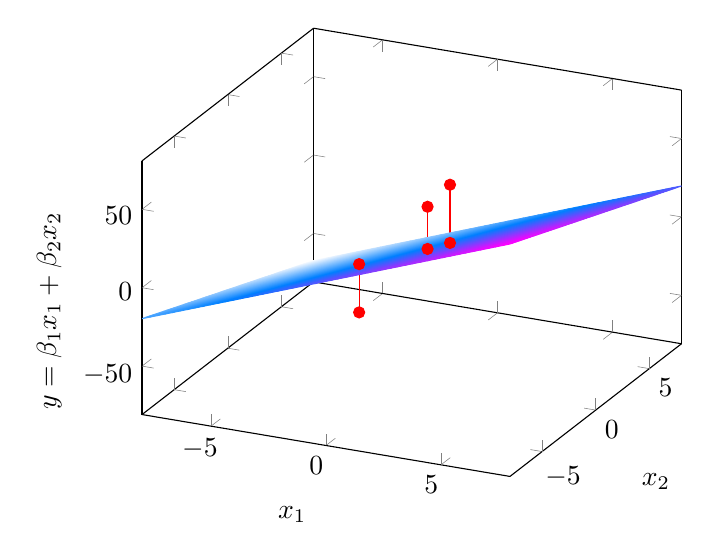
\begin{tikzpicture}
\begin{axis}[
    xlabel=$x_{1}$, ylabel=$x_{2}$, zlabel={$y=\beta_{1}x_{1}+\beta_{2}x_{2}$},
    colormap/cool
] 
\addplot3[color=red,mark=*] coordinates {(0.6313521,0.1178614,30)   (0.6313521,0.1178614,3.087642) };
\addplot3[color=red,mark=*]  coordinates {(1.1409802,1.1187348,40)   (1.1409802,1.1187348,2.881960)  };
\addplot3[color=red,mark=*]  coordinates {(-1.9300577,-0.7696159,-39) (-1.9300577,-0.7696159,-8.219724)};


\addplot3[
    mesh,
    samples=50,
    domain=-8:8,
]
{5.446613*x+-2.978828*y};

\end{axis}
\end{tikzpicture}
\end{enumerate}


\end{description}

\end{document}
